\documentclass[a4paper, 12pt]{report}

\usepackage[dvipsnames]{xcolor}

%%%%%%%%%%%%%%%%
% Set Variables %
%%%%%%%%%%%%%%%%

\def\useItalian{0}  % 1 = Italian, 0 = English

\def\courseName{Graph Theory}

\def\coursePrerequisites{\begin{itemize} \item Progettazione degli Algoritmi \end{itemize}}

\def\book{TODO}

% \def\authorName{Simone Bianco}
% \def\email{bianco.simone@outlook.it}
% \def\github{https://github.com/Exyss/university-notes}
% \def\linkedin{https://www.linkedin.com/in/simone-bianco}

\def\authorName{Alessio Bandiera}
\def\email{alessio.bandiera02@gmail.com}
\def\github{https://github.com/aflaag-notes}
\def\linkedin{https://www.linkedin.com/in/alessio-bandiera-a53767223}

%%%%%%%%%%%%
% Packages %
%%%%%%%%%%%%

\usepackage{../../packages/Nyx/nyx-packages}
\usepackage{../../packages/Nyx/nyx-styles}
\usepackage{../../packages/Nyx/nyx-frames}
\usepackage{../../packages/Nyx/nyx-macros}
\usepackage{../../packages/Nyx/nyx-title}
\usepackage{../../packages/Nyx/nyx-intro}

%%%%%%%%%%%%%%
% Title-page %
%%%%%%%%%%%%%%

\logo{../../packages/Nyx/logo.png}

\if\useItalian1
    \institute{\curlyquotes{\hspace{0.25mm}Sapienza} Università di Roma}
    \faculty{Ingegneria dell'Informazione,\\Informatica e Statistica}
    \department{Dipartimento di Informatica}
    \ifdefined\book
        \subtitle{Appunti integrati con il libro \book}
    \fi
    \author{\textit{Autore}\\\authorName}
\else
    \institute{\curlyquotes{\hspace{0.25mm}Sapienza} University of Rome}
    \faculty{Faculty of Information Engineering,\\Informatics and Statistics}
    \department{Department of Computer Science}
    \ifdefined\book
        \subtitle{Lecture notes integrated with the book \book}
    \fi
    \author{\textit{Author}\\\authorName}
\fi


\title{\courseName}
\date{\today}

% \supervisor{Linus \textsc{Torvalds}}
% \context{Well, I was bored\ldots}

\addbibresource{./references.bib}

%%%%%%%%%%%%
% Document %
%%%%%%%%%%%%

\begin{document}
    \maketitle

    % The following style changes are valid only inside this scope 
    {
        \hypersetup{allcolors=black}
        \fancypagestyle{plain}{%
        \fancyhead{}        % clear all header fields
        \fancyfoot{}        % clear all header fields
        \fancyfoot[C]{\thepage}
        \renewcommand{\headrulewidth}{0pt}
        \renewcommand{\footrulewidth}{0pt}}

        \romantableofcontents
    }

    \introduction

    %%%%%%%%%%%%%%%%%%%%%

    \chapter{Basics of Graph Theory}

    placeholder \todo{write a small introduction on graph theory}

    \section{Introduction}

    \begin{frameddefn}{Graph}
        A \tbf{graph} is a pair $G = (V, E)$, where $V$ is the --- finite --- set of \tbf{vertices} of the graph, and $E$ is the set of \tbf{edges}.
    \end{frameddefn}

    For now, will assume to be working with \tbf{simple} and \tbf{undirected} graphs, i.e. graphs in which the set of edges is defined as follows $$E \subseteq [V]^2 = \{\{x, y\} \mid x, y \in V \land x \neq v\}$$ where the notation $\{x, y\}$ will be used to indicate an edge between two nodes $x, y \in V$, and will be replaced with $xy = yx$ directly --- the \tit{set} notation for edges is used to highlight that edges have no direction. We will indicate with $n$ and $m$ the cardinality of $\abs V$ and $\abs E$, respectively.

    \begin{figure}[H]
        \centering
        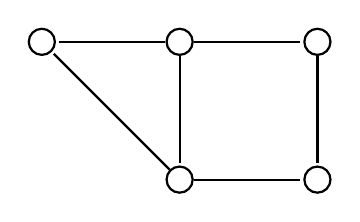
\begin{tikzpicture}[-,>=stealth,shorten >=1pt,auto,node distance=1.75cm, thick,main node/.style={scale=0.9,circle,draw,font=\sffamily\normalsize}]

            \node[circle, draw] (1) []{};
            \node[circle, draw] (2) [right of = 1]{};
            \node[circle, draw] (3) [below of = 1]{};
            \node[circle, draw] (4) [below of = 2]{};
            \node[circle, draw] (5) [left of = 1]{};

            \draw[-] (1) to (2);
            \draw[-] (1) to (3);
            \draw[-] (2) to (4);
            \draw[-] (1) to (5);
            \draw[-] (3) to (4);
            \draw[-] (3) to (5);

            ;
        \end{tikzpicture}
        \caption{A simple graph.}
        \label{first graph}
    \end{figure}

    Note that, in this definition, we are assuming that each edge has exactly 2 \tit{distinct} endpoints --- i.e. the graphs do not admit \tbf{loops} --- and there cannot exist two edges with the same endpoints. In fact, if we drop these assumption we obtain what is called a \tbf{multigraph}.

    \begin{figure}[H]
        \centering
        \begin{tikzpicture}[-,>=stealth',shorten >=1pt,auto,node distance=3cm,thick,main node/.style={scale=0.6,circle,draw,font=\sffamily\normalsize},every loop/.style={}]
            \node[main node] (1) {};
            \node[main node] (2) [below left of=1] {};
            \node[main node] (3) [below right of=2] {};

            \draw[-] (1) edge [bend left] (2);
            \draw[-] (1) edge [bend right](2);
            \draw[-] (2) edge (3);
            \draw[-] (3) edge (1);
            \draw[-] (3) edge [loop below] (3);

            ;
        \end{tikzpicture}
        \caption{A multigraph.}
    \end{figure}

    \begin{frameddefn}{Subgraph}
        Given a graph $G = (V, E)$, a \tbf{subgraph} $G' = (V', E')$ of $G$ is a graph  such that $V' \subseteq V$ and $E' \subseteq E$.
    \end{frameddefn}

    \begin{figure}[H]
        \centering
        \begin{tikzpicture}[-,>=stealth,shorten >=1pt,auto,node distance=1.75cm, thick,main node/.style={scale=0.9,circle,draw,font=\sffamily\normalsize}]

            \node[circle, draw] (1) []{};
            \node[circle, draw] (2) [right of = 1]{};
            % \node[circle, draw] (3) [below of = 1]{};
            \node[circle, draw] (4) [below of = 2]{};
            \node[circle, draw] (5) [left of = 1]{};

            % \draw[-] (1) to (2);
            % \draw[-] (1) to (3);
            % \draw[-] (2) to (4);
            \draw[-] (1) to (5);
            % \draw[-] (3) to (4);
            % \draw[-] (3) to (5);

            ;
        \end{tikzpicture}
        \caption{This is a subgraph of the graph shown in \cref{first graph}.}
    \end{figure}

    \begin{frameddefn}{Induced subgraph}
        Given a graph $G = (V, E)$, a subgraph $G' = (V', E')$ of $G$ is \tbf{induced} if every edge of $G$ with both ends in $V$ is an edge of $V'$.
    \end{frameddefn}

    This definition is \tit{stricter} than the previous one: in fact, the last graph is \tit{not} an example of an induced subgraph, but the following is:

    \begin{figure}[H]
        \centering
        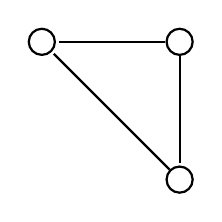
\begin{tikzpicture}[-,>=stealth,shorten >=1pt,auto,node distance=1.75cm, thick,main node/.style={scale=0.9,circle,draw,font=\sffamily\normalsize}]

            \node[circle, draw] (1) []{};
            % \node[circle, draw] (2) [right of = 1]{};
            \node[circle, draw] (3) [below of = 1]{};
            % \node[circle, draw] (4) [below of = 2]{};
            \node[circle, draw] (5) [left of = 1]{};

            % \draw[-] (1) to (2);
            \draw[-] (1) to (3);
            % \draw[-] (2) to (4);
            \draw[-] (1) to (5);
            % \draw[-] (3) to (4);
            \draw[-] (3) to (5);

            ;
        \end{tikzpicture}
        \caption{This is an \tit{induced} subgraph of the graph shown in \cref{first graph}.}
        \label{induced subgraph first graph}
    \end{figure}

    Note that every induced subgraph of a graph is \tbf{unique} by definition, and we indicate each induced subgraph as follows: suppose that the graph in \cref{first graph} had the following \tit{labeling} on the vertices

    \begin{figure}[H]
        \centering
        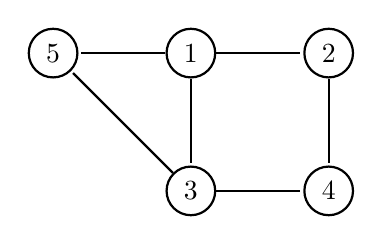
\begin{tikzpicture}[-,>=stealth,shorten >=1pt,auto,node distance=1.75cm, thick,main node/.style={scale=0.9,circle,draw,font=\sffamily\normalsize}]

            \node[circle, draw] (1) []{1};
            \node[circle, draw] (2) [right of = 1]{2};
            \node[circle, draw] (3) [below of = 1]{3};
            \node[circle, draw] (4) [below of = 2]{4};
            \node[circle, draw] (5) [left of = 1]{5};

            \draw[-] (1) to (2);
            \draw[-] (1) to (3);
            \draw[-] (2) to (4);
            \draw[-] (1) to (5);
            \draw[-] (3) to (4);
            \draw[-] (3) to (5);

            ;
        \end{tikzpicture}
        % \caption{This is an \tit{induced} subgraph of the graph shown in \cref{first graph}.}
    \end{figure}

    then, the induced subgraph in \cref{induced subgraph first graph} would have been referred to as $G[\{1, 2, 5\}]$.

    Intuitively, two vertices $x, y \in V$ are said to be \tbf{adjacent}, if there is an edge $xy \in E$, and we write $x \sim y$. If there is no such edge, we write $x \nsim y$ for non-adjacency. The \tbf{neighborhood} of a vertex $x \in V$ is the set of vertices that are adjacent to $x$, and it will be indicated as follows $$\mathcal N (x) := \{y \in V \mid x \sim y\}$$ The \tbf{degree} of a vertex $x \in V$, denoted with $\deg(x)$, is exactly $\abs{\mathcal N (x)}$. We will use the following notation for the \tbf{minimum} and \tbf{maximum} degree of a graph, respectively

    \begin{center}
        \begin{tabular}{ccc}
            $\displaystyle \delta := \min_{x \in V}{\deg(x)}$ & \qquad & $\displaystyle \Delta := \max_{x \in V}{\deg(x)}$
        \end{tabular}
    \end{center}

    \begin{framedlem}{Handshaking lemma}
        Given a graph $G = (V, E)$, it holds that $$\sum_{x \in V}{\deg(x)} = 2 \abs E$$
    \end{framedlem}

    \begin{proof}
        Trivially, the sum of the degrees counts every edge in $E$ exactly twice, once for each of the 2 endpoints.
    \end{proof}

    \begin{frameddefn}{$k$-regular graph}
        A graph $G$ is said to be \tbf{$k$-regular} if every vertex of $G$ has degree $k$.
    \end{frameddefn}

    Note that in a $k$-regular graph it holds that $$\sum_{x \in V}{\deg(x)} = k \cdot n$$

    \begin{framedprop}{}
        There are no $k$-regular graphs with $k$ odd and an odd number of vertices.
    \end{framedprop}
    
    \begin{proof}
        By way of contradiction, suppose that there exists a $k$-regular graph $G = (V, E)$ such that both $k$ and $n$ are odd; however, by the handshaking lemma we would get that $$2 \abs E = \sum_{x \in V} {\deg(x)} = k \cdot n$$ but the product of two odd numbers, namely $k$ and $n$, is still an odd number, while $2 \abs E$ must be even $\lightning$.
    \end{proof}

    \subsection{Important structures}

    \begin{frameddefn}{Path}
        A \tbf{path} is a \tit{graph} with vertex set $x_0, \ldots, x_n$ and edge set $e_1, \ldots, e_n$ such that $e_i = x_{i - 1}x_i$.

        The \tbf{length} of a path is the number of edges between $x_0$ and $x_n$, i.e. $\abs{\{e_1, \ldots, e_n\}}$, namely $n$ in this case. A path of length 1 is called \tit{trivial} path.
    \end{frameddefn}

    \begin{figure}[H]
        \centering
        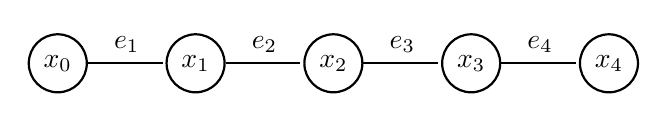
\begin{tikzpicture}[-,>=stealth,shorten >=1pt,auto,node distance=1.75cm, thick,main node/.style={scale=0.9,circle,draw,font=\sffamily\normalsize}]

            \node[circle, draw] (1) []{$x_0$};
            \node[circle, draw] (2) [right of = 1]{$x_1$};
            \node[circle, draw] (3) [right of = 2]{$x_2$};
            \node[circle, draw] (4) [right of = 3]{$x_3$};
            \node[circle, draw] (5) [right of = 4]{$x_4$};

            \draw[-] (1) to node[above]{$e_1$} (2);
            \draw[-] (2) to node[above]{$e_2$} (3);
            \draw[-] (3) to node[above]{$e_3$} (4);
            \draw[-] (4) to node[above]{$e_4$} (5);

            ;
        \end{tikzpicture}
        \caption{A path graph of length 4 that links $x_0$ and $x_4$.}
    \end{figure}

    \begin{frameddefn}{Walk}
        Given a graph $G = (V, E)$, a \tbf{walk} is a \tit{sequence} of vertices and edges $$x_0 \ e_1 \ x_1 \ \ldots \ x_{k - 1} \ e_k \ x_k$$ where $x_0, \ldots, x_k \in V$, $e_1, \ldots, e_k \in E$ and $e_i = x_{i - 1}x_i$.

        The \tbf{length} of a walk is the number of edges between $x_0$ and $x_k$, i.e. $\abs{\{e_1, \ldots , e_k \}}$, namely $k$ in this case. If $x_0 = x_k$ we say that the walk is \tbf{closed}.
    \end{frameddefn}

    If there is a path -- or a walk --- between two vertices $x, y \in V$, we say that the path --- or the walk --- \tbf{links} $x$ and $y$, and we write this as $x \to y$. For instance, given the previous graph labeled as follows

    \begin{figure}[H]
        \centering
        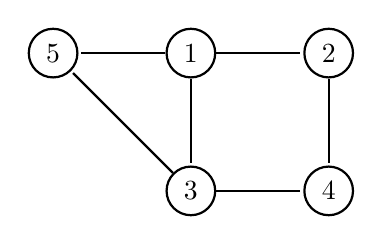
\begin{tikzpicture}[-,>=stealth,shorten >=1pt,auto,node distance=1.75cm, thick,main node/.style={scale=0.9,circle,draw,font=\sffamily\normalsize}]

            \node[circle, draw] (1) []{1};
            \node[circle, draw] (2) [right of = 1]{2};
            \node[circle, draw] (3) [below of = 1]{3};
            \node[circle, draw] (4) [below of = 2]{4};
            \node[circle, draw] (5) [left of = 1]{5};

            \draw[-] (1) to (2);
            \draw[-] (1) to (3);
            \draw[-] (2) to (4);
            \draw[-] (1) to (5);
            \draw[-] (3) to (4);
            \draw[-] (3) to (5);

            ;
        \end{tikzpicture}
        % \caption{Giv}
    \end{figure}

    an example of a walk over this graph is given by the following sequence $$1 \ \{1, 2\} \ 2 \ \{2, 4\} \ 4 \ \{4, 3\} \ 3 \ \{3, 1\} \ 1 \ \{1, 5\} \ 5$$ that \tit{links} 1 and 5, i.e. the walk is of the form $1 \to 5$.

    Note that there is a subtle difference between the definitions of \tbf{path} and \tbf{walk}: the definition of a path implies that this is always a \tit{graph} on its own, while a walk is defined as a \tit{sequence}. Nonetheless, we will treat \tit{paths} as if they where \tit{sequences} as well. This assumption holds for the following structures that will be discussed as well.

    However, by definition of path, not every alternating sequence of vertices and edges is a valid path, in fact:
    
    \begin{itemize}
        \item in a \tit{walk} it is possible to repeat both vertices and edges
        \item in a \tit{path} there can be no repetition of vertices nor edges (note that \tit{edge} repetition implies \tit{vertex} repetition)
    \end{itemize}

    For instance, the previous example of \tit{walk} is not a valid \tit{path}, because the vertex 1 is repeated.

    \begin{framedprop}{}
        Given a graph $G = (V, E)$ and two vertices $x, y \in V$, in $G$ there is a path $x \to y$ if and only if there is a walk $x \to y$.
    \end{framedprop}

    \begin{proof}
        By definition, every path is a walk, thus the direct implication is trivially true. To prove the converse implication, consider two vertices $x$ and $y$ for which there is at least one walk $x \to y$ in $G$. Now, out of all the possible walks $x \to y$ in $G$, consider the \tit{shortest} one, i.e. the one with the least amount of edges, and let it be the following sequence $$x \ e_1 \ x_1 \ \ldots \ x_{k - 1} \ e_k \ y $$ By way of contradiction, assume that this walk is not a path. Therefore, there must be either one vertex or one edge repeated, but since edge repetition always implies vertex repetition, we just need to take this case into account. Assume that there are two indices $i, j \in [k - 1]$ such that $i \neq j$ and $x_i = x_j$; however this implies that $$x \ e_1 \ \ldots \ x_{i - 1} \ e_i \ x_i \ e_{j + 1} \ x_{j + 1} \ \ldots \ x_{k - 1} \ e_k \ y$$ is still a walk $x \to y$ of strictly shorter length, but we chose the original sequence to be the \tit{shortest} possible walk $x \to y$ $\lightning$.
    \end{proof}

    \begin{framedprop}{}
        Every graph has a path of length at least $\delta$.
    \end{framedprop}
    
    \begin{proof}
        Consider a graph $G = (V, E)$, and let $P$ be $G$'s \tit{longest} path, labeled as follows $$x_0 \ e_1 \ x_1 \ \ldots \ x_{k - 1} \ e_k \ x_k$$ and assume that its length is $k$. Since $P$ is the longest path of $G$, $x_k$ cannot have neighbors outside $P$ itself, otherwise $P$ would not have been the longest path of $G$ --- it could have been extended by one of $x_k$'s neighbors. This implies that $$\mathcal N(x_k) \subseteq \{x_0, \ldots, x_{k - 1}\}$$ and since $\delta \le \deg(x_k) := \abs{\mathcal N(x_k)}$ by definition of $\delta$, this implies that $$\delta \le \abs{\{x_0, \ldots, x_{k - 1}\}} = k$$ which implies that this path is at least $\delta$-long, as desired.
    \end{proof}

    \begin{frameddefn}{Cycle}
        A \tbf{cycle} is a \tit{graph} with vertex set $x_1, \ldots, x_n$ and edge set $x_1x_2, x_2x_3, \ldots, x_{n- 1}x_n, x_nx_1$.

        The \tbf{length} of a cycle is the number of edges between $x_1$ and $x_n$, namely $n$ in this case.
    \end{frameddefn}

        \begin{figure}[H]
        \centering
        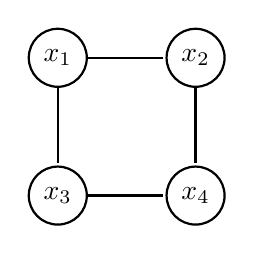
\begin{tikzpicture}[-,>=stealth,shorten >=1pt,auto,node distance=1.75cm, thick,main node/.style={scale=0.9,circle,draw,font=\sffamily\normalsize}]

            \node[circle, draw] (1) []{$x_1$};
            \node[circle, draw] (2) [right of = 1]{$x_2$};
            \node[circle, draw] (3) [below of = 1]{$x_3$};
            \node[circle, draw] (4) [below of = 2]{$x_4$};

            \draw[-] (1) to (2);
            \draw[-] (1) to (3);
            \draw[-] (2) to (4);
            \draw[-] (3) to (4);

            ;
        \end{tikzpicture}
        \caption{A cycle graph of length 4.}
    \end{figure}

    A graph that does not admit cycle subgraphs --- or \tit{cycles}, for short --- is said to be \tbf{acyclic}.

    \begin{framedprop}[label={min deg 2}]{}
        Every graph such that $\delta \ge 2$ has a cycle of length at least $\delta + 1$.
    \end{framedprop}

    \begin{proof}
        TODO \todo{qualcosa non torna}
    \end{proof}

    \begin{frameddefn}{Connected graph}
        An undirected graph $G = (V, E)$ is said to be \tbf{connected} if and only if for each vertex pair $x, y \in V$ there is a path $x \to y$.
    \end{frameddefn}

    All the graphs that we presented so far are \tit{connected}, thus the following figure provides an example of an \tbf{disconnected} graph.

    \begin{figure}[H]
        \centering
        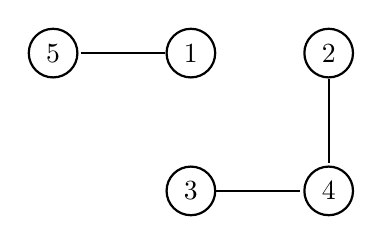
\begin{tikzpicture}[-,>=stealth,shorten >=1pt,auto,node distance=1.75cm, thick,main node/.style={scale=0.9,circle,draw,font=\sffamily\normalsize}]

            \node[circle, draw] (1) []{1};
            \node[circle, draw] (2) [right of = 1]{2};
            \node[circle, draw] (3) [below of = 1]{3};
            \node[circle, draw] (4) [below of = 2]{4};
            \node[circle, draw] (5) [left of = 1]{5};

            % \draw[-] (1) to (2);
            % \draw[-] (1) to (3);
            \draw[-] (2) to (4);
            \draw[-] (1) to (5);
            \draw[-] (3) to (4);
            % \draw[-] (3) to (5);

            ;
        \end{tikzpicture}
        % \caption{An disconnected graph.}
    \end{figure}

    \begin{frameddefn}{Component}
        Given a graph $G$, a \tbf{component} of $G$ is a maximal connected subgraph of $G$.
    \end{frameddefn}

    For instance, the graph of the previous example is made up of 2 components, namely the following two subgraphs $$C_1 = (\{1, 5\}, \{\{1, 5\}\})$$ $$C_2 = (\{2, 3, 4\}, \{\{2, 4\}, \{4, 3\}\})$$

    \begin{framedprop}[label={avoid cycle}]{}
        If $G$ is a connected graph, and $C$ is a cycle in $G$, then for any edge $e \in C$ it holds that $G - \{e\}$ is still connected.
    \end{framedprop}

    \begin{proof}
        placeholder \todo{non ho voglia ora}
    \end{proof}

    \begin{frameddefn}{Tree}
        A \tbf{tree} is a connected acyclic graph. Usually, but not necessarily, there is a fixed vertex called \tbf{root}, and any vertex that has degree 1 in the tree is called \tbf{leaf}.
    \end{frameddefn}
    
    \begin{figure}[H]
        \centering
        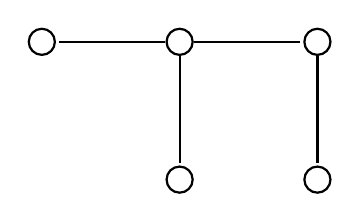
\begin{tikzpicture}[-,>=stealth,shorten >=1pt,auto,node distance=1.75cm, thick,main node/.style={scale=0.9,circle,draw,font=\sffamily\normalsize}]

            \node[circle, draw] (1) []{};
            \node[circle, draw] (2) [right of = 1]{};
            \node[circle, draw] (3) [below of = 1]{};
            \node[circle, draw] (4) [below of = 2]{};
            \node[circle, draw] (5) [left of = 1]{};

            \draw[-] (1) to (2);
            \draw[-] (1) to (3);
            \draw[-] (2) to (4);
            \draw[-] (1) to (5);
            % \draw[-] (3) to (4);
            % \draw[-] (3) to (5);

            ;
        \end{tikzpicture}
        \caption{A tree with tree leaves.}
    \end{figure}

    A \tbf{forest} is an disconnected graph, in which each component is a \tit{tree}, as in the following example

    \begin{figure}[H]
        \centering
        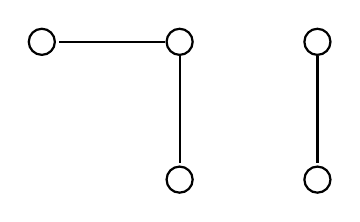
\begin{tikzpicture}[-,>=stealth,shorten >=1pt,auto,node distance=1.75cm, thick,main node/.style={scale=0.9,circle,draw,font=\sffamily\normalsize}]

            \node[circle, draw] (1) []{};
            \node[circle, draw] (2) [right of = 1]{};
            \node[circle, draw] (3) [below of = 1]{};
            \node[circle, draw] (4) [below of = 2]{};
            \node[circle, draw] (5) [left of = 1]{};

            % \draw[-] (1) to (2);
            \draw[-] (1) to (3);
            \draw[-] (2) to (4);
            \draw[-] (1) to (5);
            % \draw[-] (3) to (4);
            % \draw[-] (3) to (5);

            ;
        \end{tikzpicture}
        \caption{A forest.}
    \end{figure}

    \begin{framedthm}{Alternative definitions of tree}
        Given a graph $T = (V, E)$, the following statements are equivalent:

        \begin{enumerate}
            \item $T$ is a tree
            \item every vertex pair of $T$ is connected by a unique path
            \item $T$ is \tit{minimally connected}, i.e. $T$ is connected and $\forall e \in E$ it holds that $T- \{e\}$ is disconnected
            \item $T$ is \tit{maximally acyclic}, i.e. $T$ is acyclic and $\forall x, y \in V$ such that $x \nsim y$, it holds that $T \cup \{xy\}$ has a cycle
        \end{enumerate}
    \end{framedthm}

    \begin{proof}
        We will prove the statements cyclically.
        \begin{itemize}
            \item $1 \implies 2$. By contrapositive, assume that in $T$ there exist two vertices $x, y \in V$ for which there are two distinct paths $P$ and $Q$ of the form $x \to y$. If $P$ and $Q$ are edge-disjoint, then $P \cup Q$ is a cycle, which implies that $T$ is not a tree by definition.

                Otherwise, assume that $P$ and $Q$ are not edge-disjoint. If we start say in $x$, and we follow $Q$ edge by edge since $P$ and $Q$ are distinct, at some point we will encounter an edge $\{u, v\}$ such that $u \in P \cap Q$ and $v \in Q - P$ --- possibly, $u = x$ itself. Moreover, since both paths lead to $y$, if we keep following $Q$ we will encounter a vertex $z \in P \cap Q$ --- possibly, $z = y$ itself --- from which the two paths will coincide. Let $Q'$ be the subpath of $P$ starting with $u$ and ending in $z$; then, $Q' \cup (Q - P)$ is a cycle in $T$, which implies that $T$ is not a tree by definition.

                \begin{figure}[H]
                    \centering
                    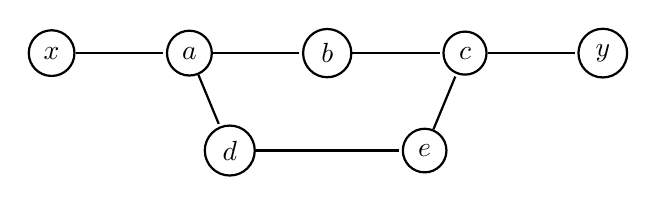
\begin{tikzpicture}[-,>=stealth,shorten >=1pt,auto,node distance=1.75cm, thick,main node/.style={scale=0.9,circle,draw,font=\sffamily\normalsize}]

                        \node[circle, draw] (1) []{$x$};
                        \node[circle, draw] (2) [right of = 1]{$a$};
                        \node[circle, draw] (3) [right of = 2]{$b$};
                        \node[circle, draw] (4) [right of = 3]{$c$};
                        \node[circle, draw] (5) [right of = 4]{$y$};
                        \node[circle, draw] (6) [below left of = 3]{$d$};
                        \node[circle, draw] (7) [below right of = 3]{$e$};

                        \draw[-] (1) to (2);
                        \draw[-] (2) to (3);
                        \draw[-] (3) to (4);
                        \draw[-] (4) to (5);
                        \draw[-] (2) to (6);
                        \draw[-] (7) to (4);
                        \draw[-] (6) to (7);

                        ;
                    \end{tikzpicture}
                    \caption{For instance, applying the argument of the proof in this graph we would get that $P = \{x, a, b, c, y\}$, $Q = \{x, a, d, e, c, y\}$, $Q - P = \{d, e\}$, $u = a$, $z = c$ and $Q' = \{a, b, c\}$, in fact $Q' \cup (Q - P) = \{a, b, c, e, d\}$ which is a cycle.}
                \end{figure}
            \item $2 \implies 3$. Consider an edge $xy \in E$; this edge itself is a path $x \to y$, and if we assume statement 2 this implies that it is the \tit{only} path from $x$ to $y$. This implies that $T - \{xy\}$ cannot contain a path from $x$ to $y$, therefore $T - \{xy\}$ is disconnected.
            \item $3 \implies 4$. Since statement 3 implies that $T$ is connected, by \cref{avoid cycle} we have that $T$ is acyclic. Now, pick $x, y \in V$ such that $x \nsim y$; by connectivity of $T$ there must be a path $x \to y$ in $T$, and let this path be $P$. Lastly, since $x \nsim y$, we have that $P \cup \{xy\}$ is a cycle in $T$.
            \item $4 \implies 1$ By contrapositive, we want to prove that if $T$ is not a tree, then $T$ is not maximally acyclic. Note that if $T$ is not a tree, we have two options:

                \begin{itemize}
                    \item if $T$ is connected but contains a cycle, then $T$ is clearly not maximally acyclic
                    \item if $T$ is acyclic but disconnected, then by definition there must exist two vertices $x, y \in V$ such that there is no path $x \to y$, which implies that $T \cup \{xy\}$ still does not contain any cycle
                \end{itemize}
        \end{itemize}
    \end{proof}

    \begin{framedprop}{}
        Every tree with at least 2 vertices has a leaf.
    \end{framedprop}
    
    \begin{proof}
        By way of contradiction, assume $T$ is a tree with at least 2 vertices that does not contain any leaves; then $\delta \ge 2$ in $T$, which implies that $T$ contains a cycle of length at least $\delta + 1$ by \cref{min deg 2}.
    \end{proof}

    \printbibliography % UNCOMMENT FOR BIBLIOGRAPHY

\end{document}
